\chapter{Deep Networks for Equalization}

The equalization process removes inter-symbol interference caused by the channel from a sequence of symbols.  We will explore how neural networks can both estimate the channel characteristics and remove the inter-symbol interference.  For the remainder of this paper, we will assume that all channels only have real parts. 

\section{Channel Estimation}

\begin{itemize}
\item compare least squares and how KNN did with pure deep nn based architecture
\item NN did better than least squares
\item hyperparam search over general 1-layer to 4-layer dense layers, and number of nodes and activations
\item plots: how error changed with respect to data points, as number of data points increased, NN outperformed LS
\item preamble: 100
\item want: QPSK, plot of preamble length
\item want? how to visualize that NN does better than LS
\end{itemize}

Plot comparing least squares to KNN to NN.



\section{Channel Equalization}

The process of equalization tries to remove inter-symbol interference from a sequence of symbols.  
In a two tap channel, the equalization process is trying to remove the effect from the second channel tap.  Given the received symbol, $\tilde{x}_m$, the channel taps, $a_0, a_1$, and the previous symbol, $x_{m-1}$, we can solve for the best estimate of the orignal symbol.
\begin{align}
\tilde{x}_m &= a_0 x_{m} + a_1 x_{m-1} + v_m\\
\hat{x}_m &= \frac{\tilde{x}_m - a_1 x_{m-1}}{a_0}
\end{align}

If we want neural networks to perform equalization, they might try to solve for $\hat{x}_m$ in this way.  
If that is the case, then the neural networks will need to know how to take and input and divide by it and how to multiply two inputs.  

\subsection{Learning an inverse}

\begin{figure}
\begin{center}
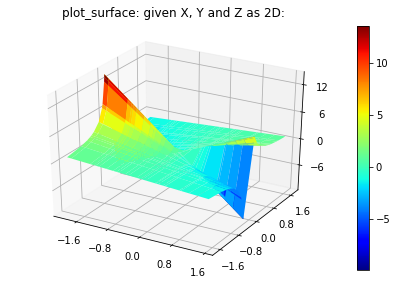
\includegraphics{figures/equal/Division_Function_plot.png}
\caption{Topographical surface representation of the division function; $z=\frac{x}{y}$.}
\label{fig:div_fx}
\end{center}
\end{figure}

\begin{figure}
\begin{center}
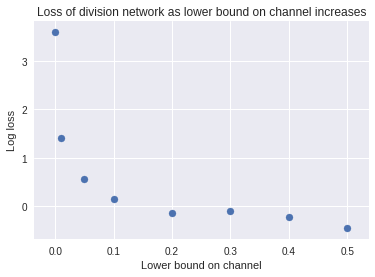
\includegraphics{figures/equal/Channel_lower_bound_division.png}
\caption{Neural network divsion with respect to the lower bound of $y$.}
\label{fig:one_tap_inv}
\end{center}
\end{figure}

We explore whether a neural network can learn to do division.  We did not do a thorough architecture search or train for very long as we wanted an idea of the behavior of the neural network and will do this in future work.  
Figure~\ref{fig:div_fx} shows the topological representation of the division function, $z=\frac{x}{y}$.  A neural network that is trained to do division will need to approximate the surface of this function.  
When $y$ is close to zero, $z$ becomes very large and goes to infinity.  These large peaks will make it difficult for a neural network to do division.  

Figure~\ref{fig:one_tap_inv} shows the performance of a neural network learning division.
The neural network's input is $x$ and $y$ and the output is $\hat{z}$.  Both inputs are uniform random variables; $x$ is drawn uniformly $[-1,1]$ and $y$ is drawn uniformly $[\beta,1]$. 
The loss function is the mean squared error between the estimated division and the true division, $\hat{z}-\frac{x}{y}$.
The architecture consists of two dense layers with $50$ nodes each and sigmoid activiation function.  This feeds into a linear layer that outputs the scalar estimate of $\hat{z}$.  
The network is re-trained with $10k$ data points for different values of $\beta$. As $\beta$ gets close to zero, the error increases dramatically.  This is expected because the closer $\beta$ is to zero, the stronger the effects are of the infinite peaks of the division function.

\subsection{Learning to multiply two inputs}

\begin{figure}
\begin{center}
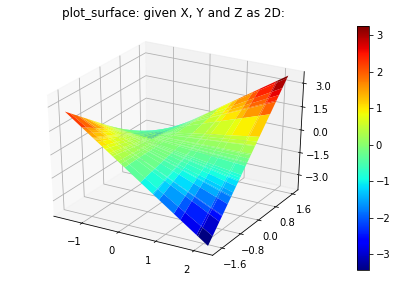
\includegraphics{figures/equal/Multiplication_Function_plot.png}
\caption{Topographical surface representation of the multiplication function; $z=xy$.}
\label{fig:mult_fx}
\end{center}
\end{figure}

%\begin{figure}
%\begin{center}
%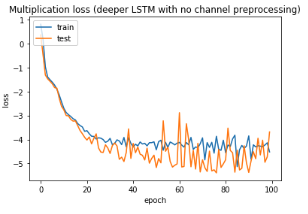
\includegraphics{figures/equal/LSTM_loss_multiplication.png}
%\caption{LSTM loss trying to learn the Multiplication function; $z=xy$.}
%\end{center}
%\label{fig:lstm_loss_mult}
%\end{figure}

%\begin{figure}
%\begin{center}
%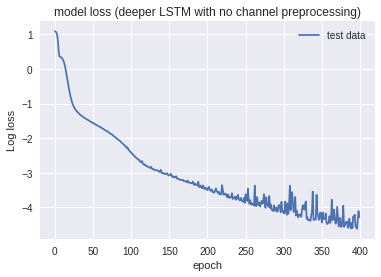
\includegraphics{figures/equal/Multiplication_loss_vs_epoch.png}
%\caption{LSTM loss trying to learn the Multiplication function; $z=xy$.}
%\end{center}
%\label{fig:loss_mult}
%\end{figure}

\begin{figure}
\begin{center}
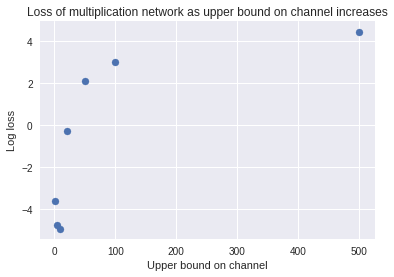
\includegraphics{figures/equal/Channel_upper_bound_multiplication.png}
\caption{Neural network divsion with respect to the upper bound of $y$.}
\label{fig:mult_bound}
\end{center}
\end{figure}

We explore whether a neural network can learn to do multiplication. We did not do a thorough architecture search or train for very long as we wanted an idea of the behavior of the neural network and will do this in future work. 
Figure~\ref{fig:mult_fx} shows the topological representation of the multiplication function, $z=xy$.  A neural network that is trained to do multiplication will need to approximate the surface of this function.  
When $x$ and $y$ are close to zero, the function is stable.  However, as $x$ and $y$ grow, the function becomes unstable and grows to infinity. 

Figure~\ref{fig:mult_bound} shows the performance of a neural network learning multiplication.
The neural network's input is $x$ and $y$ and the output is $\hat{z}$.  Both inputs are uniform random variables; $x$ is drawn uniformly $[-1,1]$ and $y$ is drawn uniformly $[0,\gamma]$. 
The loss function is the mean squared error between the estimated multiplication and the true multiplication, $\hat{z}-xy$.
The architecture consists of two dense layers with $50$ nodes each and sigmoid activiation function.  This feeds into a linear layer that outputs the scalar estimate of $\hat{z}$.  
The network is re-trained with $50k$ data points for different values of $\gamma$. As $\gamma$ increases, the error increases dramatically.  This is expected because the larger $\gamma$ is, the stronger the effects are of the infinite limits of the multiplication function.


\subsection{RNN for Channel Equalization}

We designed an RNN to perform channel equalization.
The inputs of the RNN are the true channel taps.  We assume a two tap channel so $a_0, a_1$ are input to the RNN.  Another input is the received data sequence, $\vec{\tilde{x}}_{data}$.
The output of the RNN is an estimate of the original data sequence, $\vec{\hat{x}}_{data}$. 
The loss function that the RNN is trained on is the mean squared error between the original and estimated data sequence, $||\vec{x}_{data}-\vec{\hat{x}}_{data}||^2$.

\begin{figure}
\begin{center}
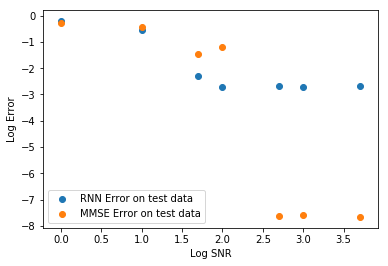
\includegraphics[width=100mm]{figures/equal/RNN_vs_MMSE.png}
\caption{Comparison of RNN and MMSE mean squared error after equalization.}
\label{fig:rnn_vs_mmse}
\end{center}
\end{figure}

The neural network architecture for our equalizer uses a special type of RNN called a bidriectional long-short term memory (LSTM) network.  
A bidirectional RNN connects the forward and backwards nodes of the RNN, allowing the output to depend on both future and past states.
An RNN that has LSTM units allows the nodes to store memory for a short period of time.
Our network also has time-distributed dense layers which are used after LSTMs to flatten the output by applying a fully connected dense layer at each time step.

The input to our RNN is the channel taps concatenated with a sequence of $10$ of the symbols.  The inputs are fed into four layers of bidirectional LSTM units.  Each layer has a state size of $90$ units for each forward and backward state.  The output of the four bidirectional LSTM layers is $180$ units for each of the $10$ sequences.  
This is then fed into two time-distributed dense layers with $180$ nodes and $100$ nodes respectively and they each have Relu activation functions. These time-distributed dense layers bring the output size down from $180$ to $100$ to $100$.  The output is then fed into one final time-distributed dense layer with $100$ nodes and linear activation.  The outputs of the RNN are $10$ equalized symbols.  


Figure~\ref{fig:rnn_vs_mmse} compares the mean squared error loss on test data for the RNN architecture defined above and the MMSE equalizer defined in the introduction.  
The RNN is trained on $40k$ data sequences, with a decaying learning rate starting at $0.01$.
The RNN and MMSE are tested on the same $10k$ data sequences.  New data is generated for each SNR and the RNN is re-trained for each SNR.  Each data sequence consits of $60$ bits modulated to $30$ complex symbols.
We assume that the RNN and MMSE both have access to the true channel chracteristics.

The RNN equalizer performs comparably to the MMSE equalizer for low SNRs and performs better than MMSE equalizer for medium SNRs.  However, the RNN equalizer performs worse than the MMSE equalizer for high SNRs.  We take a closer look at what kind of channels the RNN equalizer is getting wrong.

\begin{figure}
\begin{center}
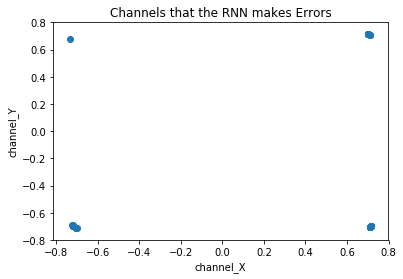
\includegraphics[width=100mm]{figures/equal/incorrect_channels.png}
\caption{What two tap channels does the equalizer get wrong?}
\label{fig:incorr_chan}
\end{center}
\end{figure}

\begin{align*}
\begin{bmatrix}
\text{Tap 1} & \text{Tap 2} & \text{Counts of bad estimates} & \text{Mean Squared Error}\\
\hline
0.707 & 0.707 & 14 & 0.7162\\
-0.707 & 0.707 & 1 & 0.5236\\
0.707 & -0.707 & 16 & 0.8172\\
-0.707 & -0.707 & 12 & 0.6492\\
\end{bmatrix}
\end{align*}

Figure~\ref{fig:incorr_chan} shows which channels the RNN equalizer and classic demodulator got any bits wrong.  
There were a total of $50k$ random channels in the test set with SNR$=100$.
Of that set, only $43$ channels resulted in incorrect bits after the RNN equalizer and classic demodulator.
From the figure, it is clear that these difficult channels are clustered into four regions. All of the four regions are when the first and second tap of the channel are equal in magnitude.
The mean squared error between the equalized data and the true data among just the bad channels was $0.7306$.  The mean squared error among the good channels was $0.000264$.


In this chapter, we designed a deep neural network to estimate two tap channels.
We explored the difficulties in learning to divide and learning to multiply with neural networks. We showed that a deep recursive neural network, with bidirectional LSTM layers, can learn to learn to equalize for random channels.  We also examined when these equalizers fail. 